\documentclass[12pt,AutoFakeBold]{article} 

\usepackage[数字信号处理]{XDULabreport}  % 载入 XDULabreport 模板文件,[]中填写科目名称,科目名称,默认为电子线路实验(I)
\problem{系统的频域和 z 域分析}  % 请在此处填写问题内容
\labdate{2021年11月05日} % 实验日期
% 其他参数在宏包中进行更改,其中学院,班级,姓名,学号均在sty宏包内进行更改
% \usepackage{fourier}  % 这是 fourier 字体,更柔和 

\newfontfamily\digi{DigifaceWide Regular} % 将数码管字体引入

%% 如果你需要中文的一级标题编号,如“一、”、“二、”等,请把下面两行取消注释
% \RequirePackage{zhnumber} % change section number to chinese
% \titleformat{\section}{\Large\bfseries\rmfamily}{\zhnum{section}、}{0em}{}

% 文档开始
        
\begin{document}

\maketitle
\setcounter{tocdepth}{2}
\tableofcontents  % 生成目录

% 正文标题
\makeatletter
\begin{center}
    \LARGE \textbf{\textsf{\@problem}}
\end{center}
\makeatother

\section{实验目的}

设计计算机程序,产生序列并计算序列的 DTFT,绘制其幅频特性和相频特性曲线;根据系统的单位脉冲响应和差分方程,计算系统的频率响应,绘制系统频率响应的幅频特性和相频特性曲线;根据系统的单位脉冲响应和差分方程,计算系统的系统系统函数、零极点分布;改变系统的零级点分布,观察系统频率响应的变化。

\section{实验原理}

\subsection{序列的离散时间傅里叶变换}

\subsubsection{DTFT 的定义}

一般序列 $x(n)$ 的 DTFT(discrete time Fourier transform) 定义为
%
\begin{equation*}
X(e^{j\omega})=\mathrm{DTFT}[x(n)]=\sum_{n=-\infty}^\infty x(n)e^{-j\omega n}
\end{equation*}
%
$X(e^{j\omega})$ 是序列 $x(n)$ 的频谱函数。上式的级数不一定总是收敛的,例如,$x(n)$ 是单位阶跃序列时级数就不收敛。序列 $x(n)$ 的 DTFT 存在的充分必要条件是序列 $x(n)$ 绝对可和,即满足
\begin{equation*}
\sum_{n=-\infty}^\infty|x(n)|<\infty
\end{equation*}

\subsubsection{DTFT 的周期性}

序列的 DTFT 定义式中,$n$ 取整数,因此
%
\begin{equation*}
X(e^{j\omega})=\sum_{n=-\infty}^\infty x(n)e^{-j(\omega+2\pi M)n},\quad M\in\mathbb{Z}
\end{equation*}
%
成立。这说明序列的 DTFT 是频率 $\omega$ 的连续周期函数,周期为 $2\pi$。由于 DTFT 的周期性,只要知道 $X(e^{j\omega})$ 的一个周期,即 $\omega\in[0,2\pi)$ 或 $\omega\in[-\pi,\pi)$,就可以分析序列的频谱,不需要取整个 $-\infty<\omega<\infty$ 域来分析。在 $\omega=0,2\pi M$ 点上,$X(e^{j\omega})$ 表示序列 $x(n)$ 的低频分量,序列 $x(n)$ 的最高频率分量在 $\omega=\pi$ 点上。

一般来说,$X(e^{j\omega})$ 是实变量 $\omega$ 的复值函数,可用实部和虚部将其表示为
%
\begin{equation*}
X(e^{j\omega})=X_R(e^{j\omega})+jX_I(e^{j\omega})
\end{equation*}
%
其中,$X_R(e^{j\omega})$、$X_I(e^{j\omega})$ 分别是 $X(e^{j\omega})$ 的实部和虚部。

$X(e^{j\omega})$ 也可以用幅度谱和相位谱表示为
%
\begin{equation*}
X(e^{j\omega})=|X(e^{j\omega})|e^{j\arg[X(e^{j\omega})]}
\end{equation*}
%
其中,$|X(e^{j\omega})$、$\arg[X(e^{j\omega})]$ 分别称为序列 $x(n)$ 的幅度谱和相位谱。

\subsection{离散时间系统 LTI 系统的频率响应}

离散时间 LTI 系统的频域特性可用系统的频率响应和系统函数进行分析。

当系统的输入是频率为 $\omega$ 的复指数序列
%
\begin{equation*}
x(n)=e^{j\omega n}
\end{equation*}
%
时,系统的零状态响应为
%
\begin{equation*}
y(n)=e^{j\omega n}*h(n)=e^{j\omega n}H(e^{j\omega})
\end{equation*}
%
式中
%
\begin{equation*}
H(e^{j\omega})=\sum_{n=-\infty}^\infty h(n)e^{-j\omega n}=\mathrm{DTFT}[h(n)]
\end{equation*}
%
$H(e^{j\omega})$ 定义为离散时间 LTI 系统的频率响应。由上式可知,复指数序列 $e^{j\omega n}$ 通过离散时间 LTI 系统后输出序列的频率不变,序列的幅度由系统的频率响应 $H(e^{j\omega})$ 在 $\omega$ 点的幅度值确定。所以 $|H(e^{j\omega})|$ 表示系统对不同频率信号的增益。

在一般情况下,离散时间系统LTI系统的频率响应 $H(e^{j\omega})$ 是复值函数,可用幅度和相位表示
%
\begin{equation*}
H(e^{j\omega})=|H(e^{j\omega})|e^{j\phi(\omega)}
\end{equation*}
%
式中,$|H(e^{j\omega})|$被称为系统的幅频响应,$\phi(\omega)$ 称为系统的相频响应。当 $h(n)$ 为实序列时,由序列的 DTFT 性质可知,$|H(e^{j\omega})|$ 是 $\omega$ 的偶函数,$\phi(\omega)$ 为 $\omega$ 的奇函数。


\section{实验过程}

实验用到了 MATLAB 和 Python 两种语言版本,具体的说明在 MATLAB 版本中,Python 版实验环境为 Jupyter Notebook,导入的包如下

\begin{lstlisting}[language=Python]
import matplotlib.pyplot as plt
import numpy as np
from scipy import signal
\end{lstlisting}

\subsection{序列的 DTFT}

\subsubsection{MATLAB 版本} \label{sec:matlab1}

我们的序列为
%
\begin{equation*}
x(n)=\begin{cases}\cos(\frac{\pi}{8}n) & n=-16,-15,\cdots,15,16\\
0& others\end{cases}
\end{equation*}
%
可以视为在区间 $[-2\pi, 2\pi]$ 对模拟信号 $y(t)=\cos(t)$ 以采样周期 $T=\frac{\pi}{8}$ 采样并将横坐标转换为 $n$ 获得,如图 \ref{fig:seq} 所示。

\begin{figure}[hbtp]
	\centering
	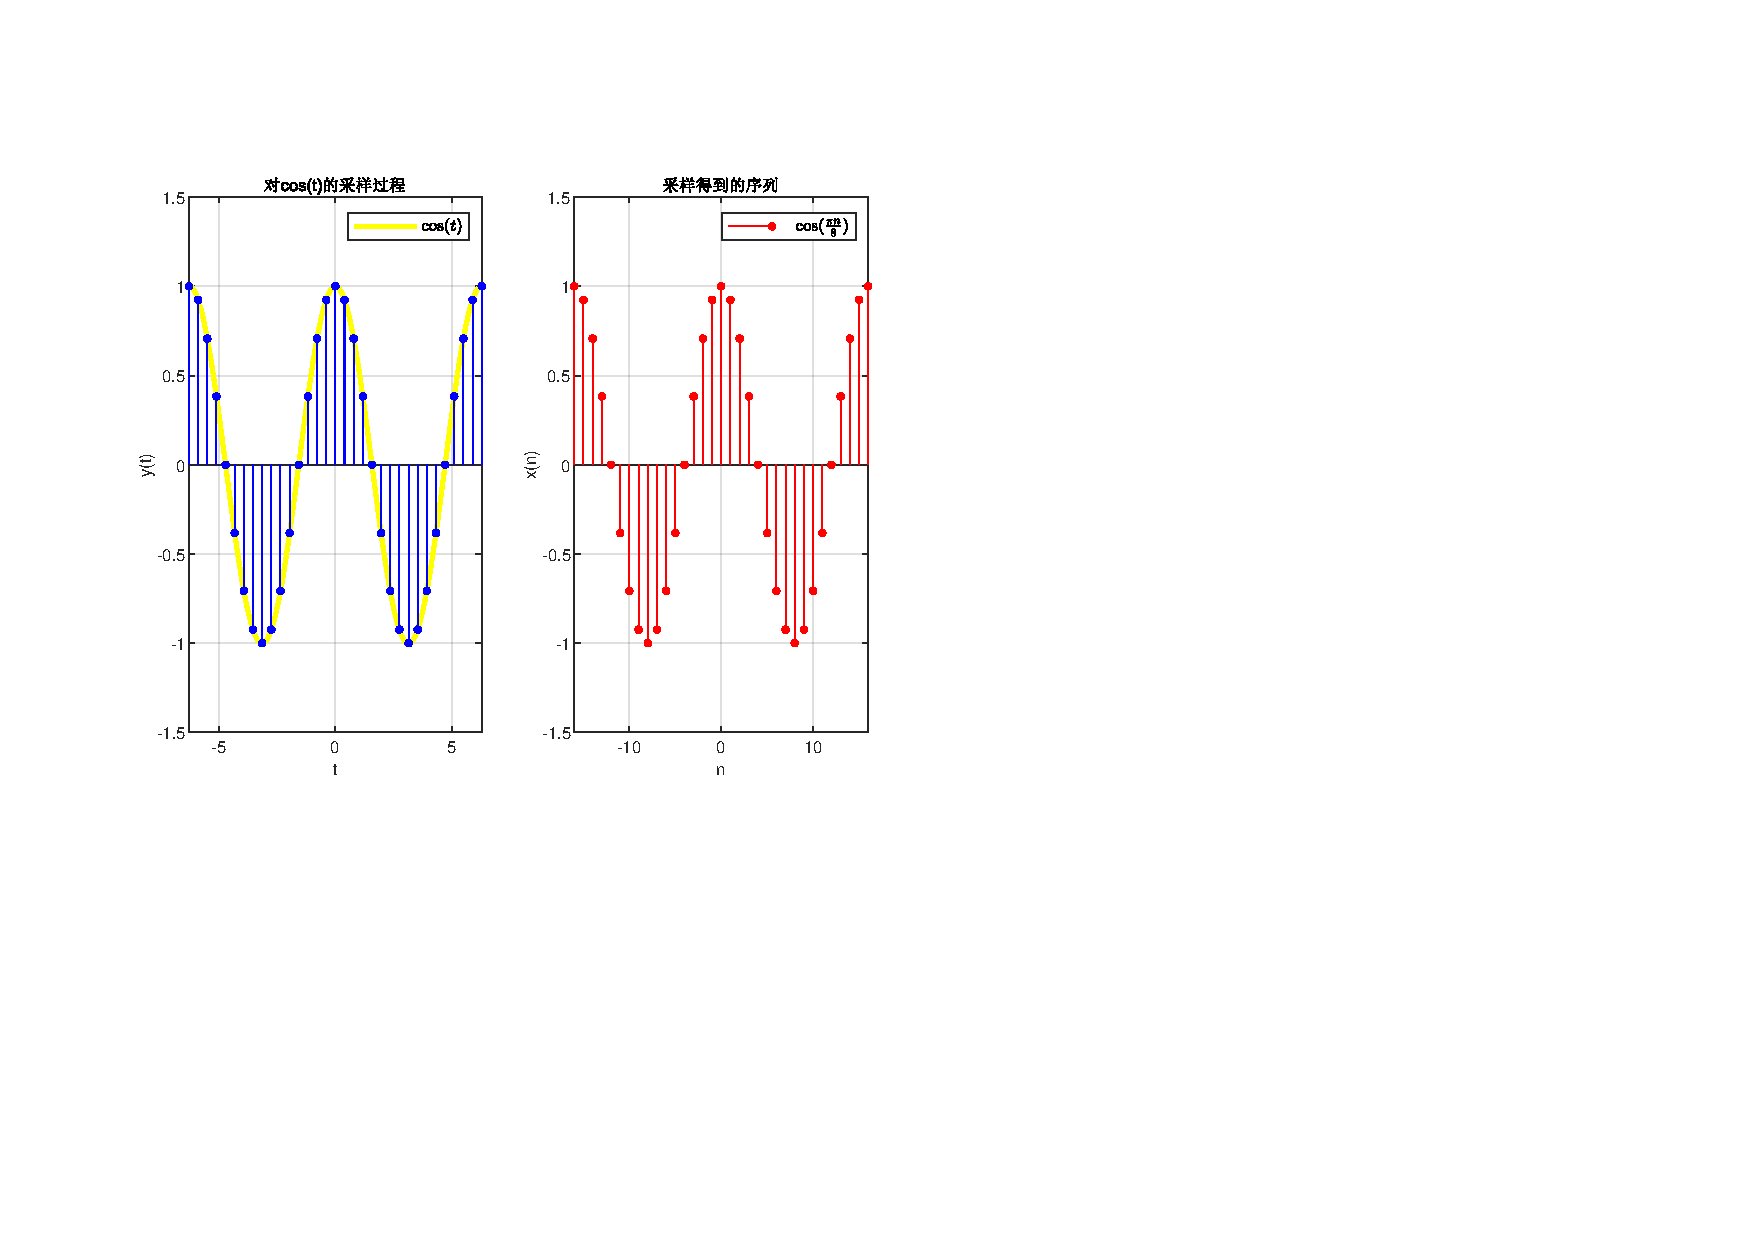
\includegraphics[width=16cm]{seq.pdf}
	\caption{序列的产生}\label{fig:seq}
\end{figure}

\begin{lstlisting}[language=Matlab]
subplot(1,2,1);
t = -2*pi:0.001:2*pi;
nt = -2*pi:2*pi/16:2*pi;
plot(t,cos(t),'y','LineWidth',2); hold on;
stem(nt,cos(nt),'b','filled','MarkerSize',3)
grid on;
axis([-2*pi 2*pi -1.5 1.5])
title('对cos(t)的采样过程');
xlabel('t');
ylabel('y(t)');
handle = legend('$\cos(t)$');
set(handle,'Interpreter','latex','FontSize',10)

subplot(1,2,2);
n = -16:16;
xn = cos(pi*n/8);
stem(n,xn,'r','filled','MarkerSize',3);
grid on;
axis([-16 16 -1.5 1.5])
title('采样得到的序列');
xlabel('n');
ylabel('x(n)');
handle = legend('$\cos(\frac{\pi n}{8})$');
set(handle,'Interpreter','latex','FontSize',10)
\end{lstlisting}

绘制得到的幅频特性和相频特性曲线如图 \ref{fig:figure1} 所示,实部和虚部曲线如图 \ref{fig:figure2} 所示。

\begin{figure}[hbtp]
	\centering
	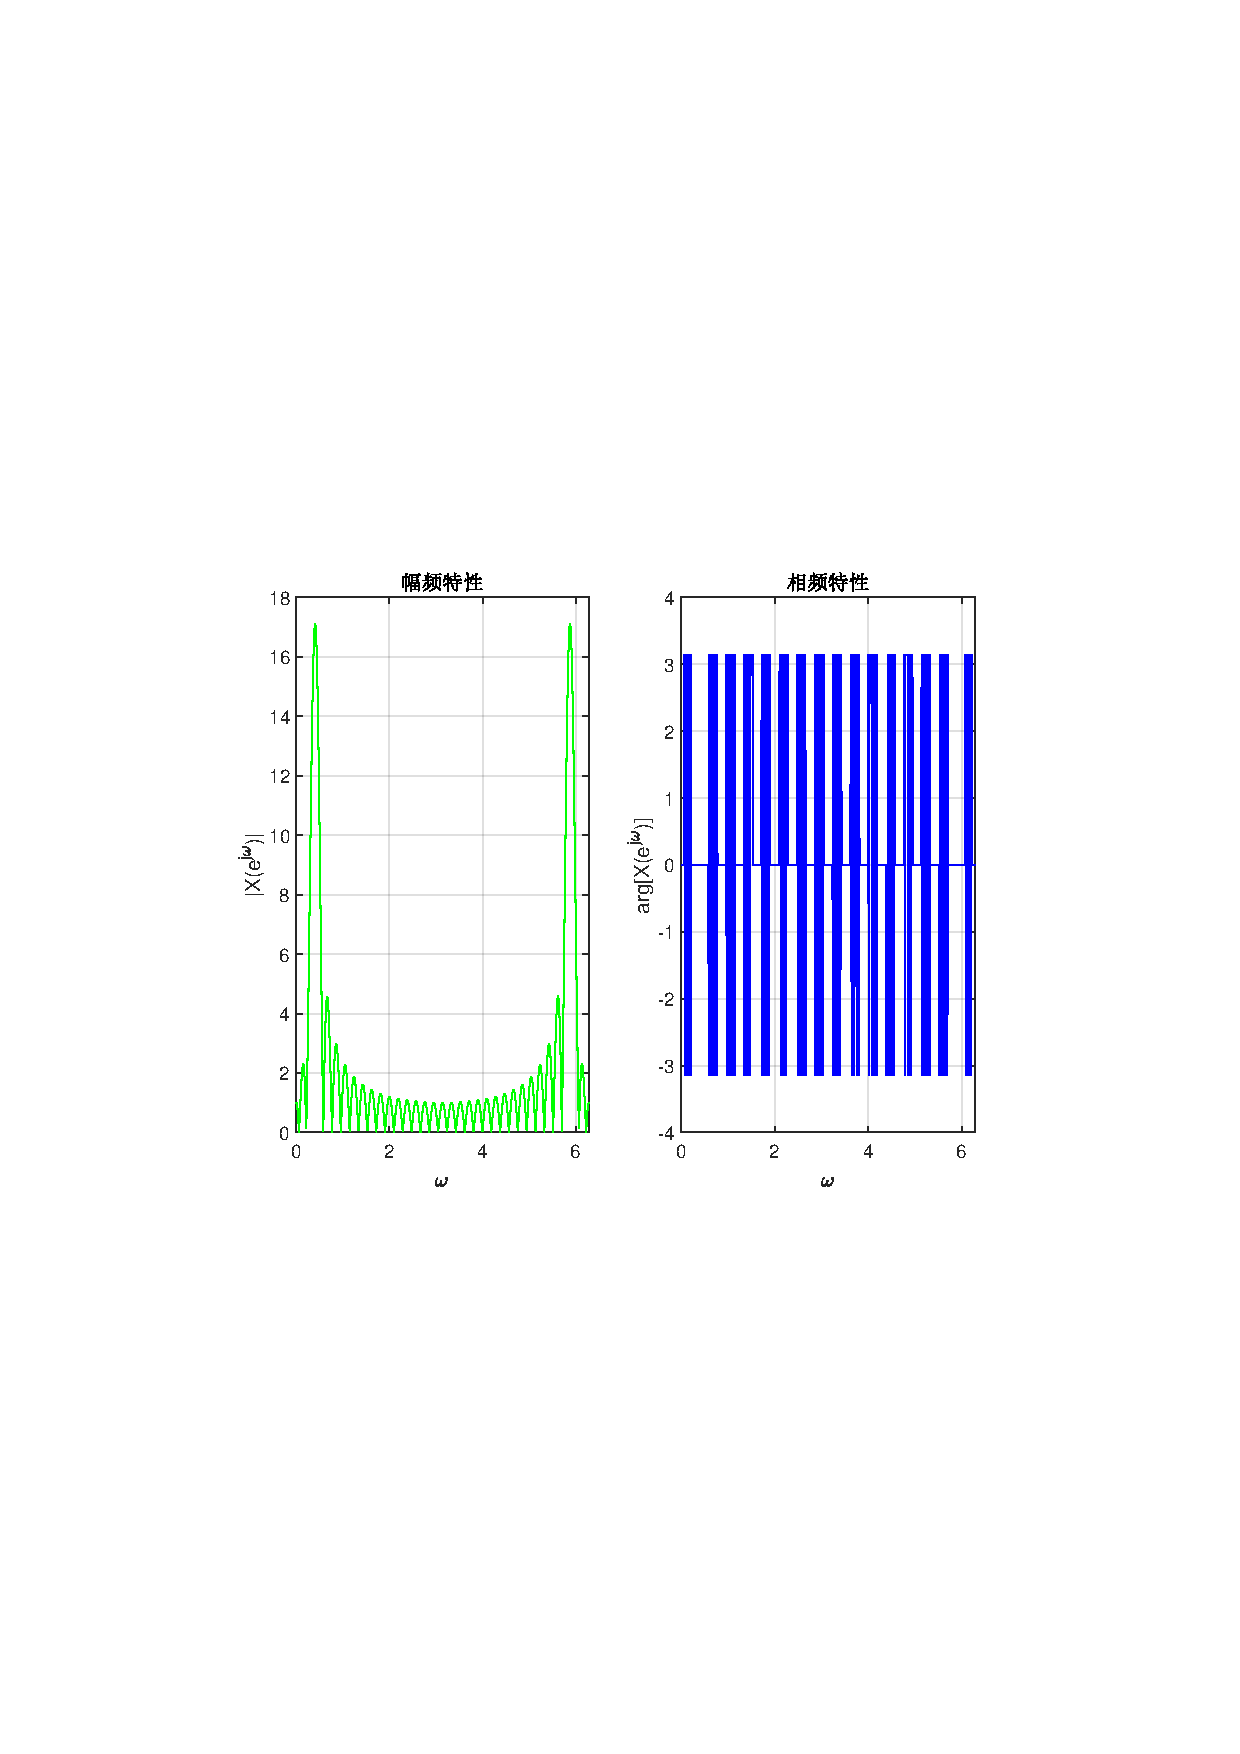
\includegraphics[width=16cm]{figure1.pdf}
	\caption{幅频特性和相频特性}\label{fig:figure1}
\end{figure}

\begin{figure}[hbtp]
	\centering
	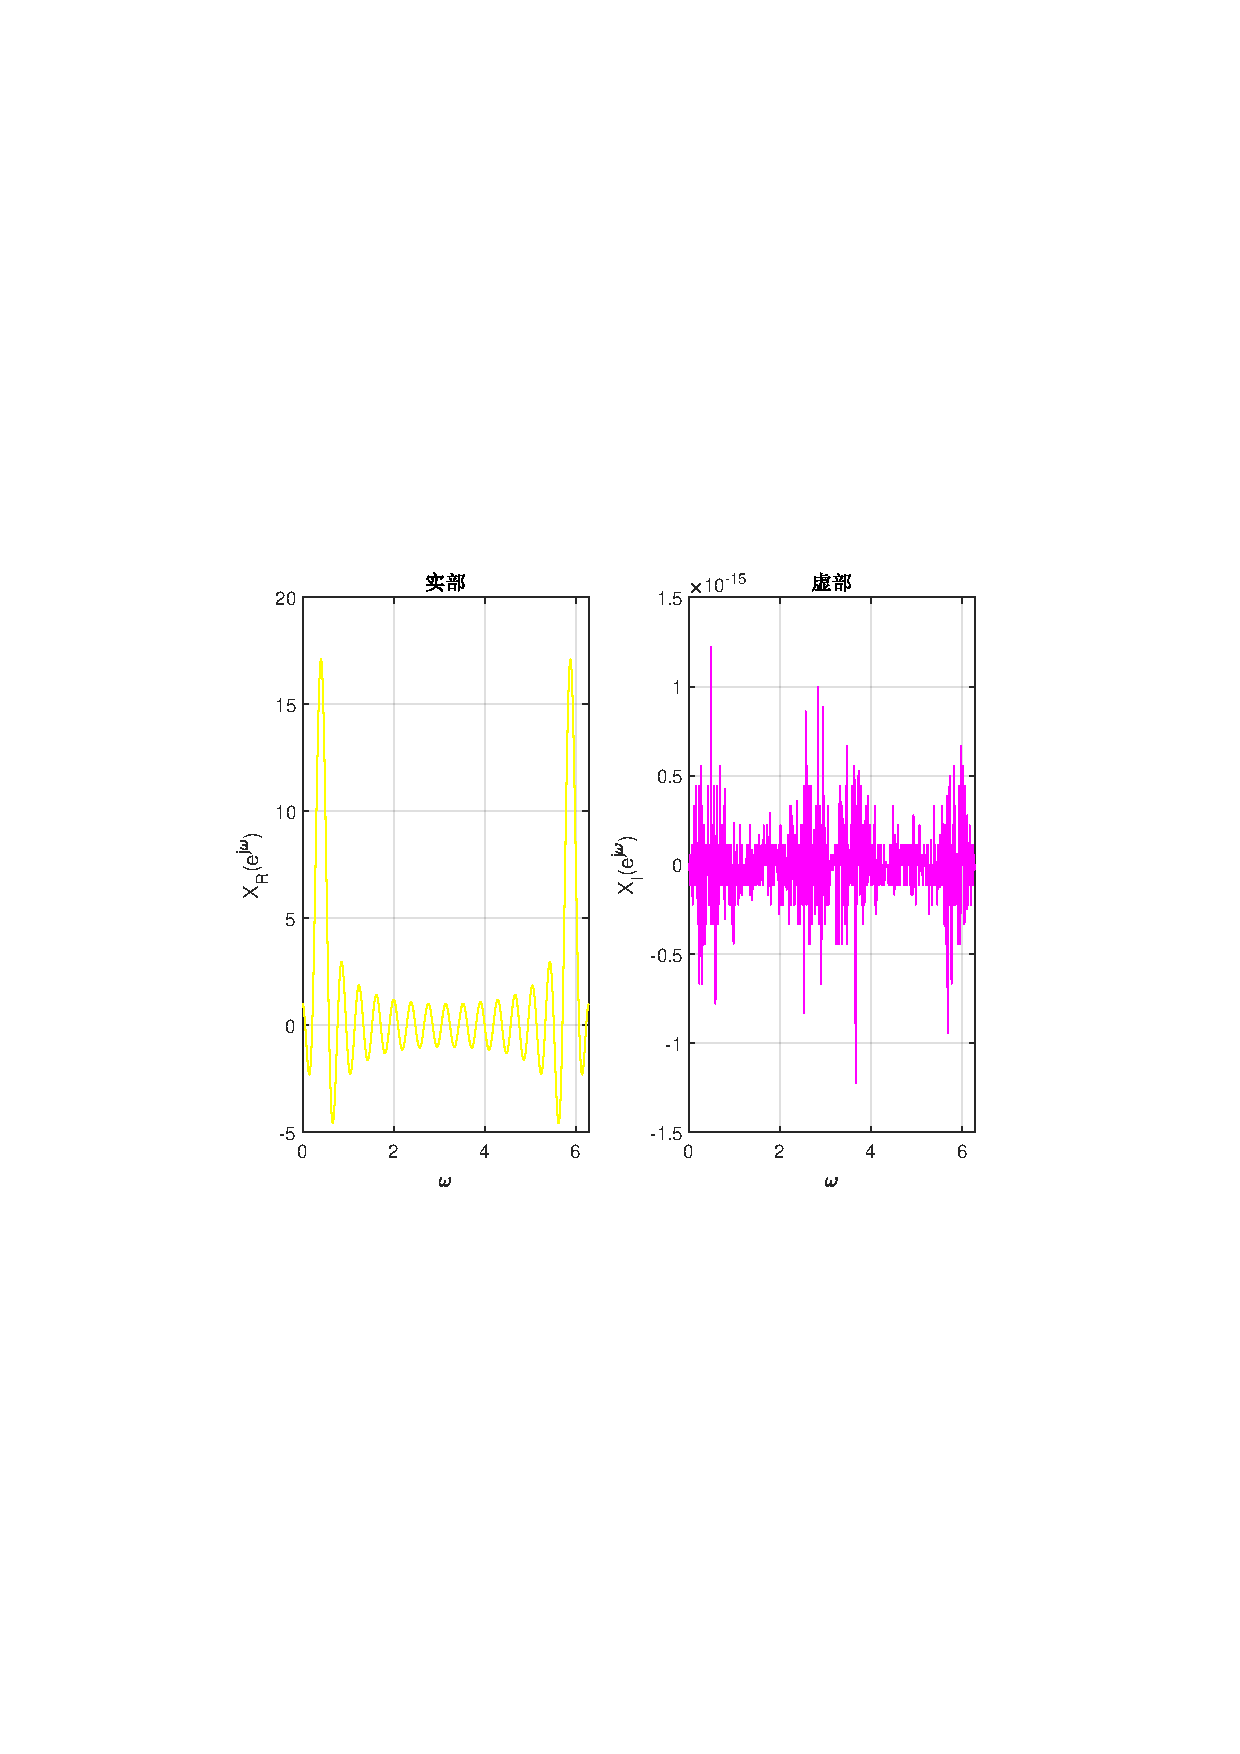
\includegraphics[width=16cm]{figure2.pdf}
	\caption{DTFT 的实部和虚部}\label{fig:figure2}
\end{figure}

\begin{lstlisting}[language=Matlab]
n = -16:16;
xn = cos(pi*n/8);
omega = linspace(0,2*pi,1000);
X = xn * exp(-j*n'*omega); % DTFT

figure(1)

subplot(1,2,1)
plot(omega,abs(X),'g')
grid on;

xlim([0 2*pi])
title('幅频特性');
xlabel('\omega');
ylabel('|X(e^{j\omega})|');

subplot(1,2,2)
plot(omega,angle(X),'b')
grid on;
title('相频特性');
xlabel('\omega');
ylabel('arg[X(e^{j\omega})]');
xlim([0 2*pi])

figure(2)

subplot(1,2,1);
plot(omega,real(X),'y')
grid on;
xlim([0 2*pi])
title('实部');
xlabel('\omega');
ylabel('X_R(e^{j\omega})');

subplot(1,2,2);
plot(omega,imag(X),'m')
grid on;
xlim([0 2*pi])
title('虚部');
xlabel('\omega');
ylabel('X_I(e^{j\omega})');
\end{lstlisting}

\subsubsection{Python 版本}

用 Python 绘制得到的幅频特性和相频特性曲线如图 \ref{fig:figure11} 所示,实部和虚部曲线如图 \ref{fig:figure2} 所示。

\begin{figure}[hbtp]
	\centering
	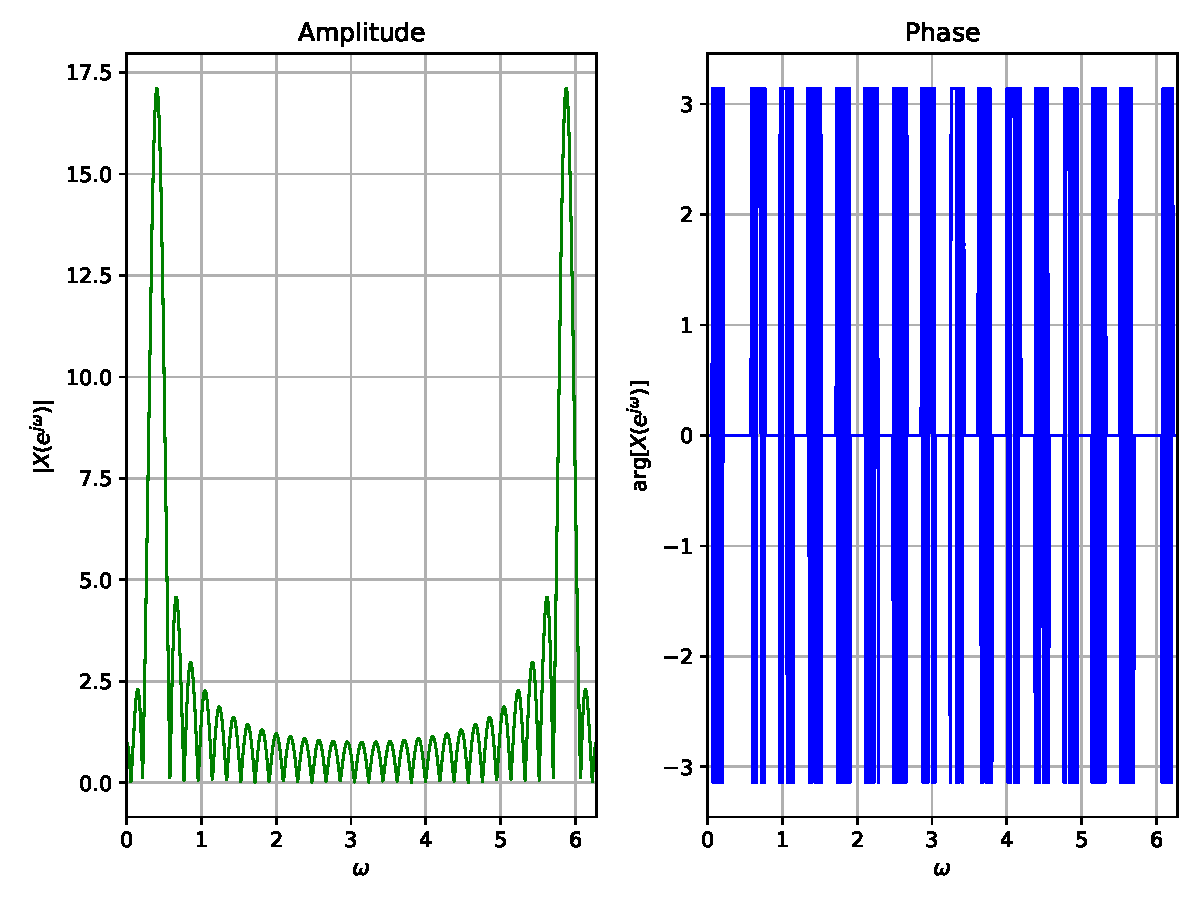
\includegraphics[width=16cm]{figure11.pdf}
	\caption{幅频特性和相频特性(Python)}\label{fig:figure11}
\end{figure}

\begin{figure}[hbtp]
	\centering
	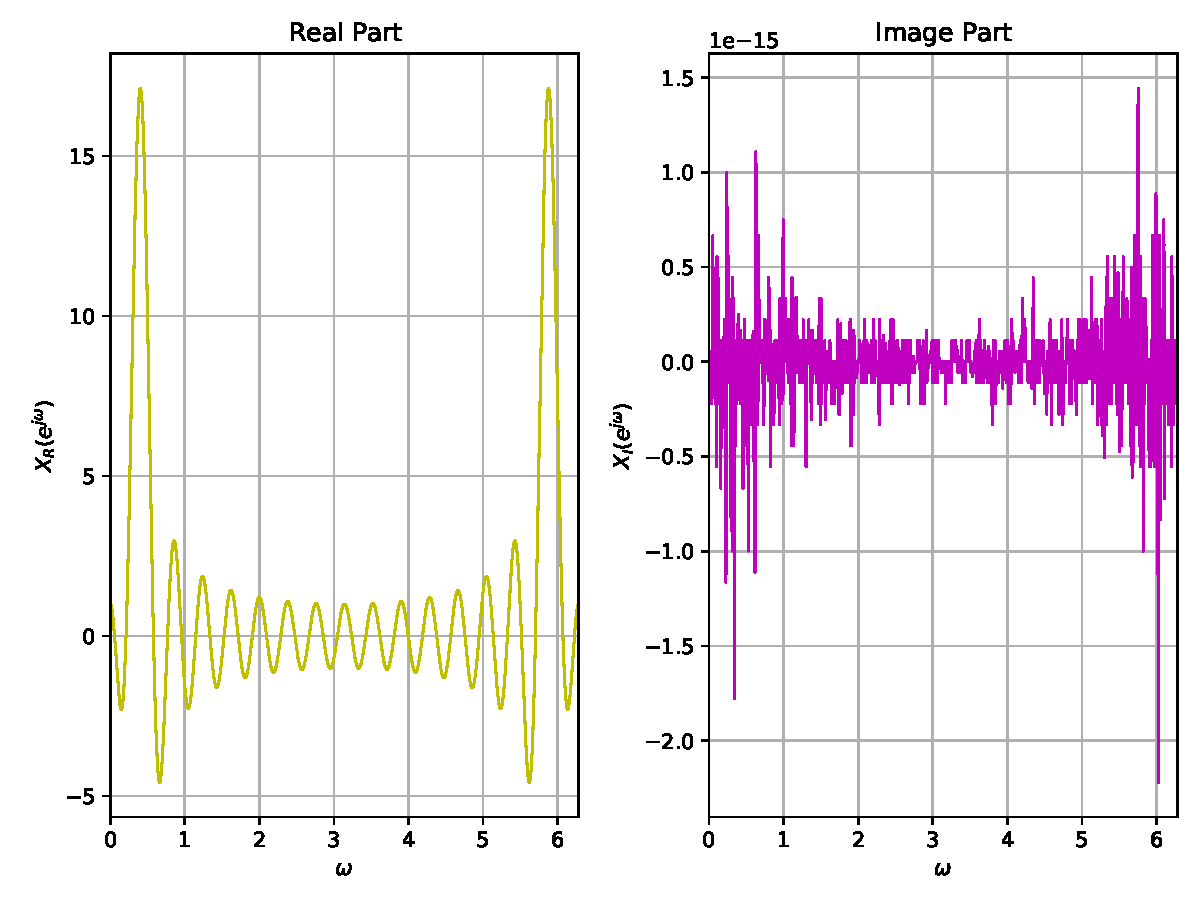
\includegraphics[width=16cm]{figure21.pdf}
	\caption{DTFT 的实部和虚部(Python)}\label{fig:figure21}
\end{figure}

\begin{lstlisting}[language=Python]
# 计算 DTFT
n = np.arange(-16,17)
n = np.mat(n)
xn = np.cos(np.pi*n/8)
omega = np.arange(0, 2*np.pi, 2*np.pi/1000)
X = xn * np.exp(-1j*n.T*omega)
X = X.T
\end{lstlisting}

\begin{lstlisting}[language=Python]
# 绘制幅频特性和相频特性曲线
plt.figure(figsize=(8, 6), dpi=80)

plt.subplot(121)
plt.plot(omega, np.abs(X), 'g', linewidth=1.0)
plt.xlim(0, 2*np.pi)
plt.grid()
plt.xlabel('$\omega$')
plt.ylabel('$|X(e^{j\omega})|$')
plt.title('Amplitude')

plt.subplot(122)
plt.plot(omega, np.angle(X), 'b', linewidth=1.0)
plt.xlim(0, 2*np.pi)
plt.grid()
plt.xlabel('$\omega$')
plt.ylabel('$\mathrm{arg}[X(e^{j\omega})]$')
plt.title('Phase')

plt.tight_layout()
plt.show()
\end{lstlisting}

\begin{lstlisting}[language=Python]
# 绘制实部和虚部曲线
plt.figure(figsize=(8, 6), dpi=80)

plt.subplot(121)
plt.plot(omega, np.real(X), 'y', linewidth=1.0)
plt.xlim(0, 2*np.pi)
plt.grid()
plt.xlabel('$\omega$')
plt.ylabel('$X_R(e^{j\omega})$')
plt.title('Real Part')

plt.subplot(122)
plt.plot(omega, np.imag(X), 'm', linewidth=1.0)
plt.xlim(0, 2*np.pi)
plt.grid()
plt.xlabel('$\omega$')
plt.ylabel('$X_I(e^{j\omega})$')
plt.title('Image Part')

plt.tight_layout()
plt.show()
\end{lstlisting}

\subsection{离散 LTI 系统的频率响应}

\subsubsection{MATLAB 版本} \label{sec:matlab2}

我们建立如下一阶系统差分方程
%
\begin{equation*}
y(n)-0.6y(n-1)=x(n)
\end{equation*}
%
其系统函数为
\begin{equation*}
H(z)=\frac{z}{z-0.6}
\end{equation*}
系统的单位脉冲响应如下,如图 \ref{fig:impz1} 所示。
\begin{equation*}
h(n)=(0.6)^nu(n)
\end{equation*}
系统函数的零点 $z=0$,极点 $p=0.6$,如图 \ref{fig:zplane1} 所示。幅频响应特性和相频响应特性如图 \ref{fig:figure3} 所示。

通过改变系统的零极点分布我们发现,当 $\omega$ 从 $0$ 变化到 $2\pi$ 时,对应单位圆上的点 B,当 B 点转到极点附近时,该极点矢量长度短,因而幅频响应出现峰值,且极点越靠近单位圆,极点矢量长度越短,峰值越高越尖锐。如果极点在单位圆上,该极点对应的幅频响应无穷大,系统是不稳定的,这与稳定系统的收敛域要包含单位圆的条件是一致的。对于零点,结果相反,当 B 点转到零点附近时,该零点矢量长度最短,幅频响应将出现谷值,零点愈靠近单位圆,谷值愈接近零。当零点处在单位圆上时,谷值为 0。

\begin{figure}[htbp]
	\centering
	\begin{minipage}[t]{0.48\textwidth}
		\centering
		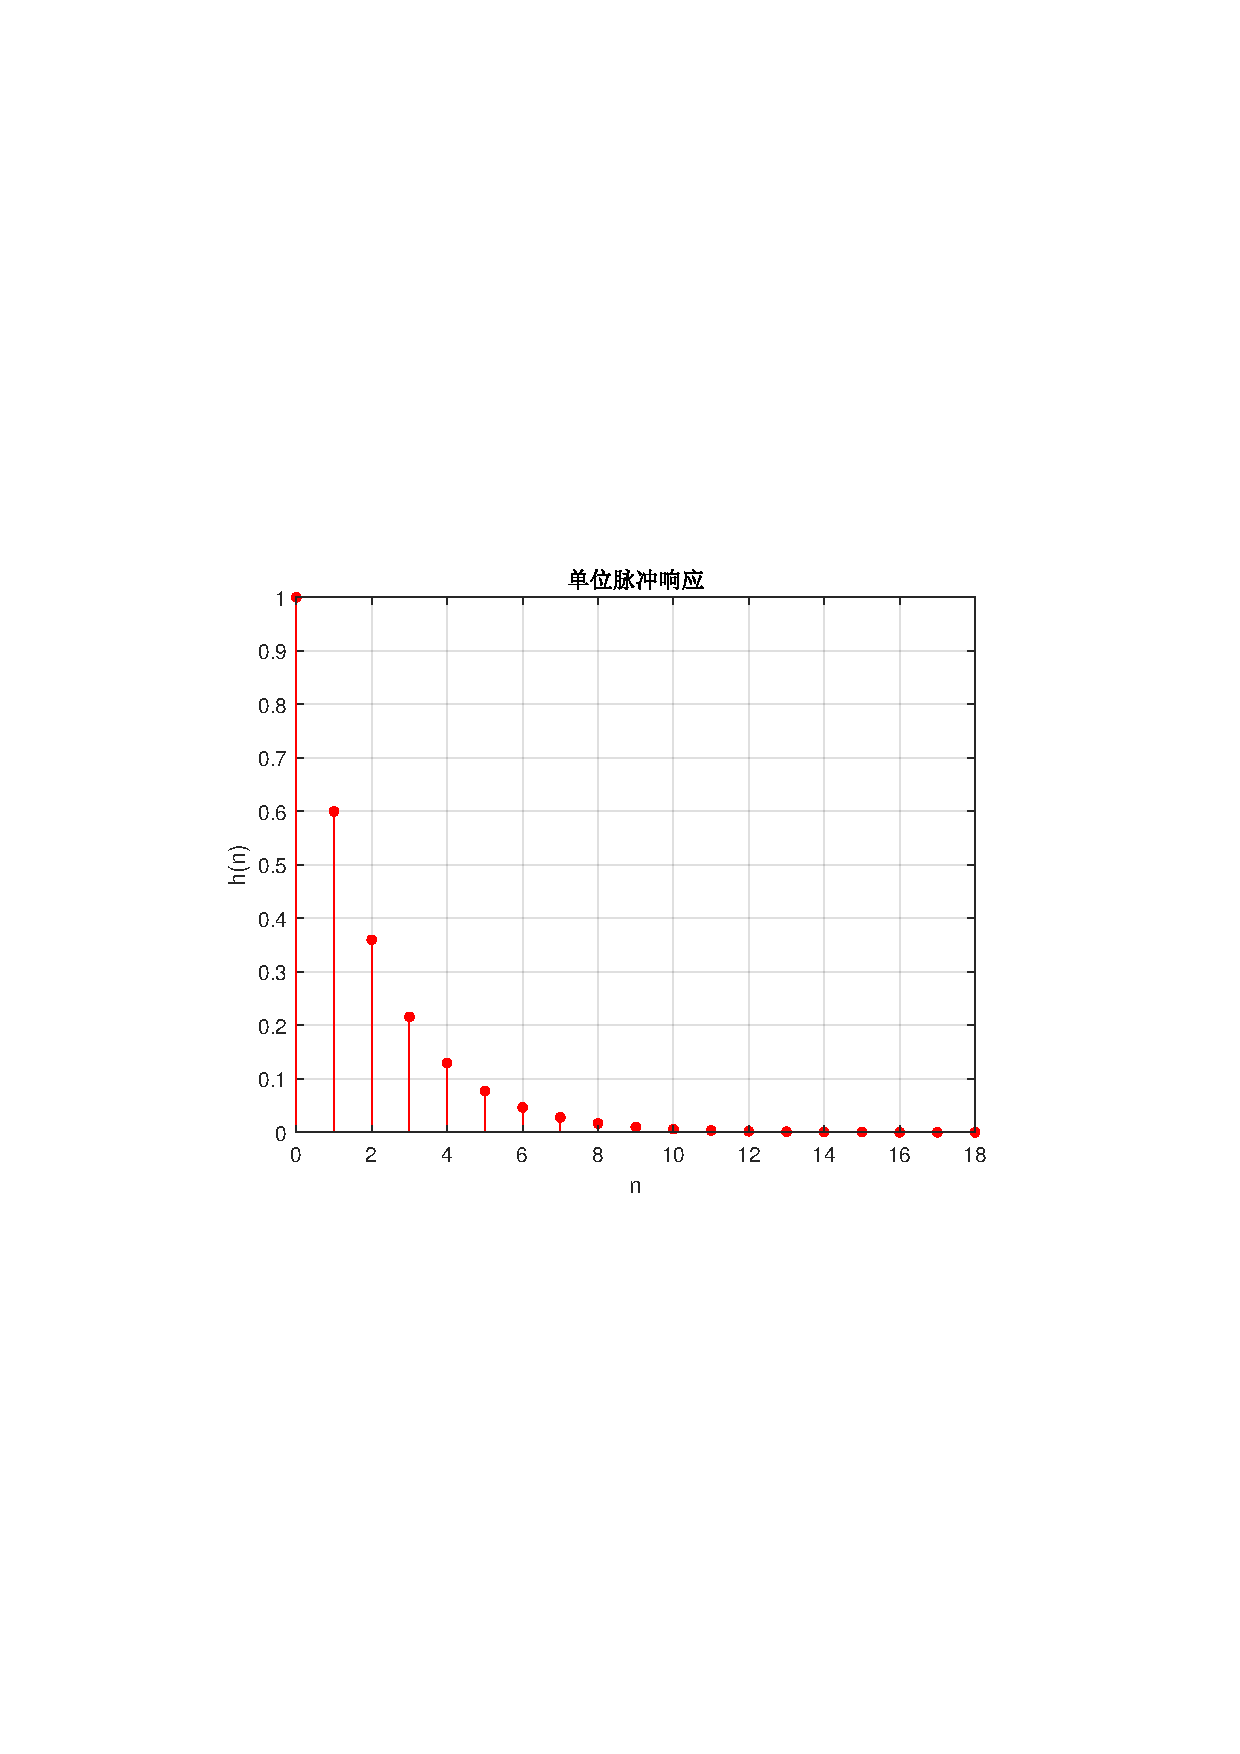
\includegraphics[width=6cm]{figure/impz1.pdf}
		\caption{单位脉冲响应}\label{fig:impz1}
	\end{minipage}
	\begin{minipage}[t]{0.48\textwidth}
		\centering
		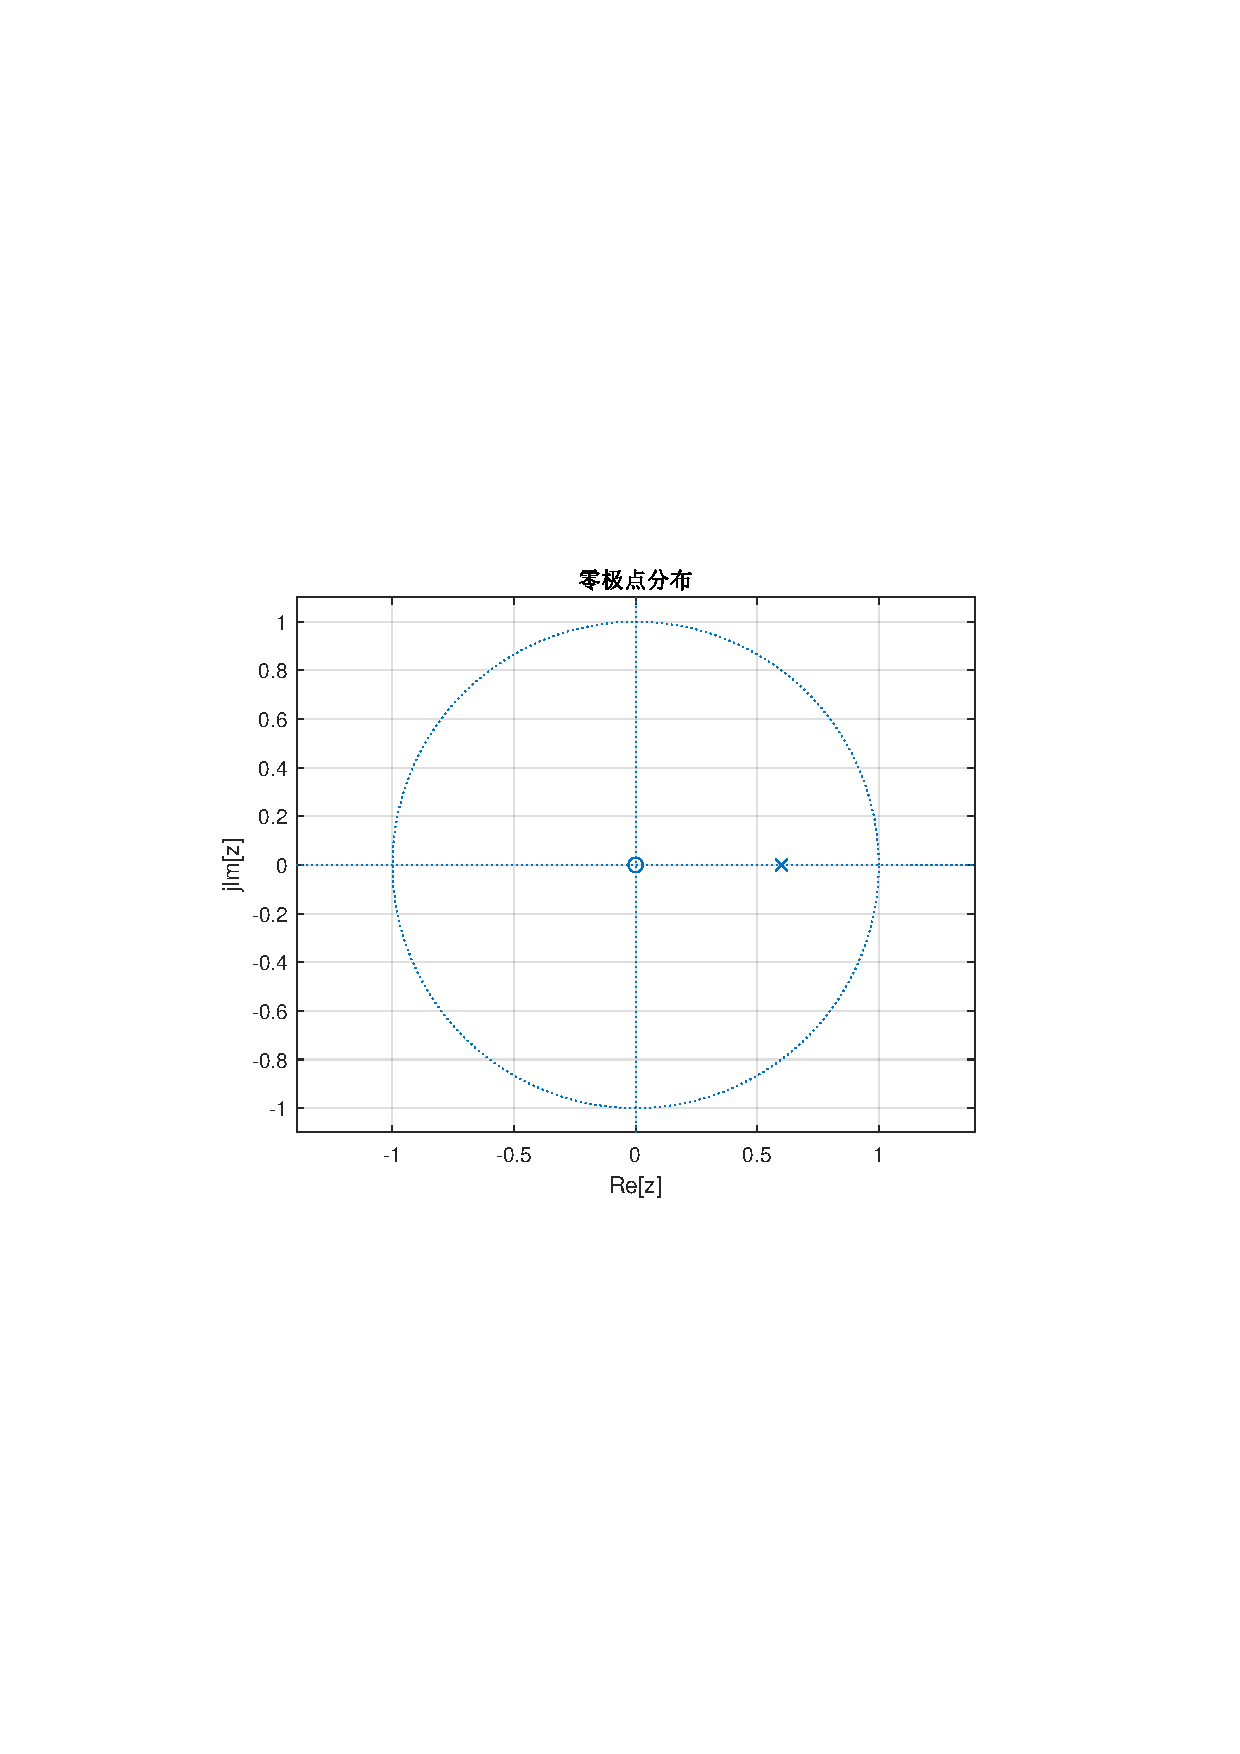
\includegraphics[width=6cm]{figure/zplane1.pdf}
		\caption{零极点分布图}\label{fig:zplane1}
	\end{minipage}
\end{figure}

\begin{figure}[hbtp]
	\centering
	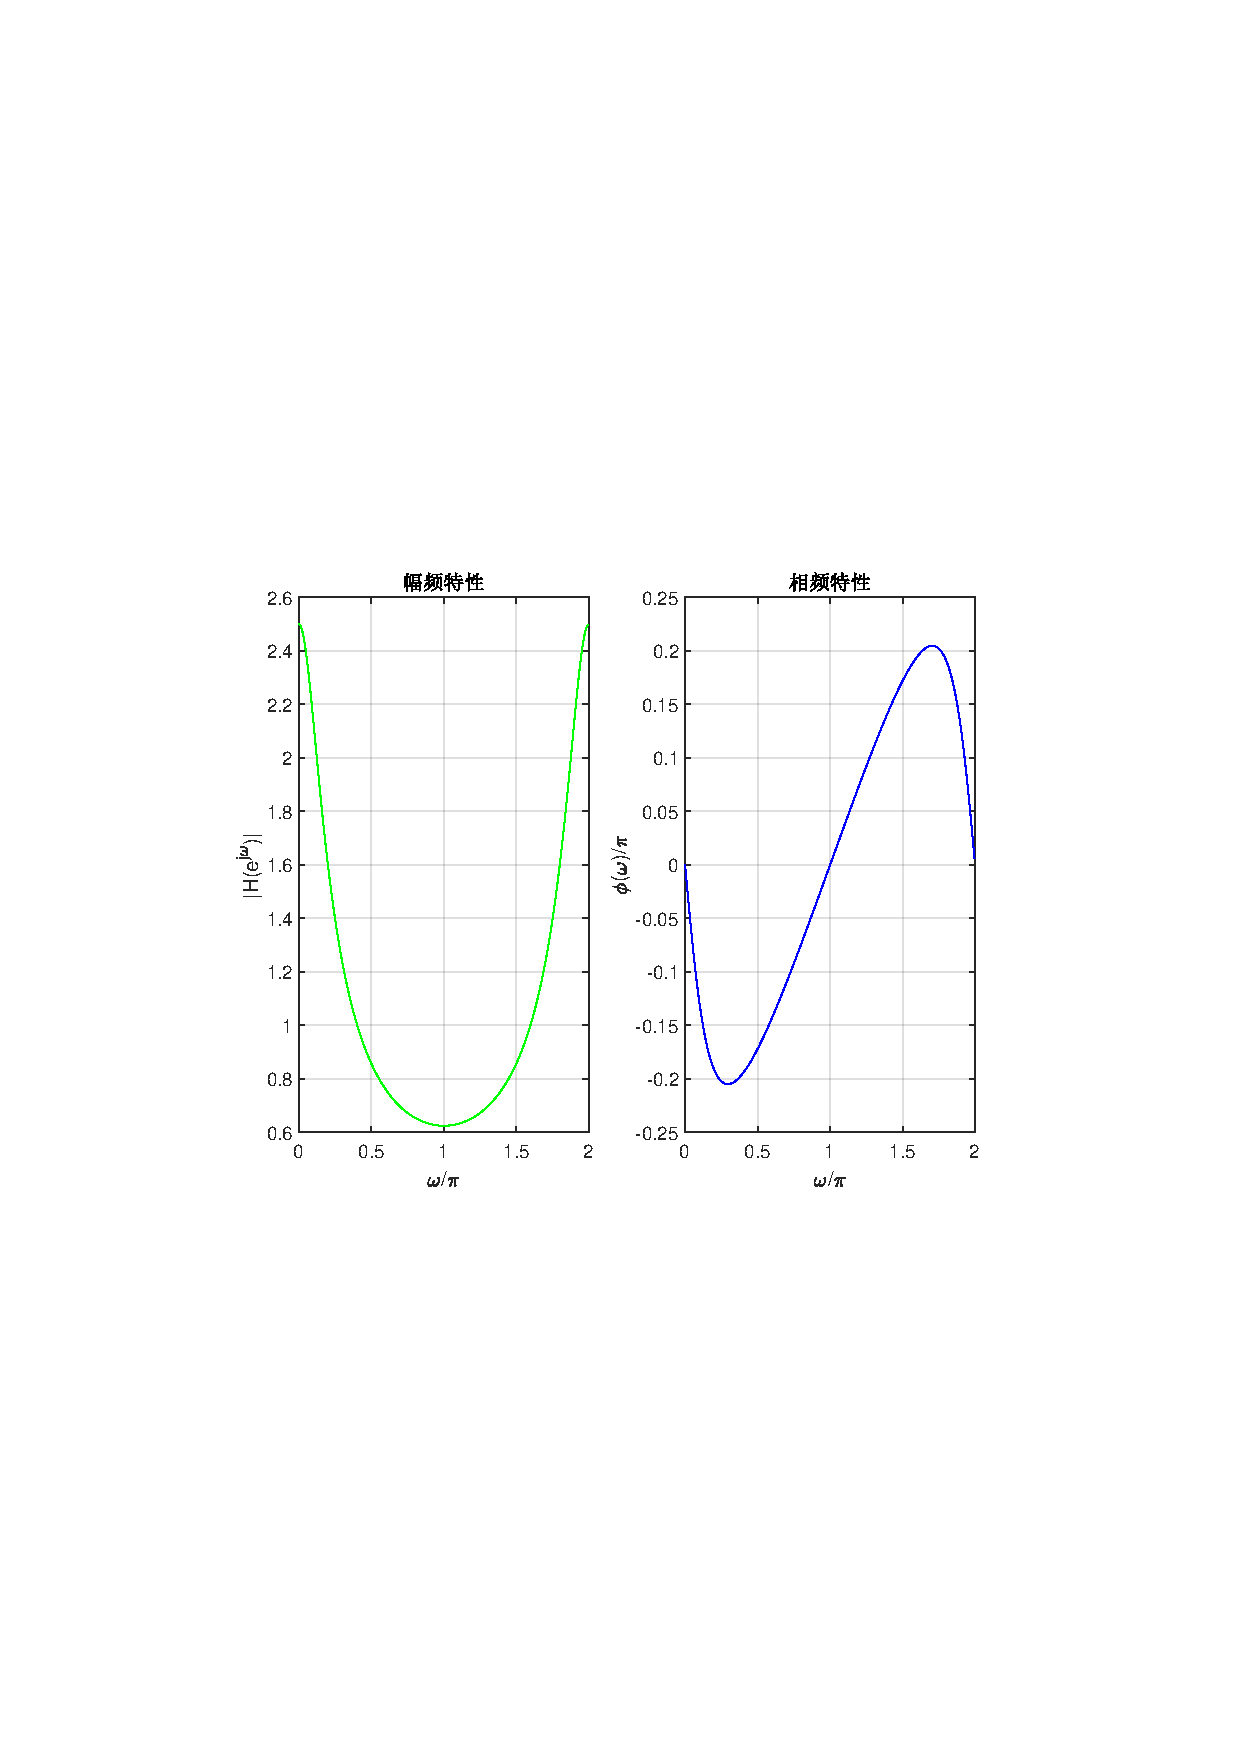
\includegraphics[width=16cm]{figure3.pdf}
	\caption{幅频特性和相频特性}\label{fig:figure3}
\end{figure}

\begin{lstlisting}[language=Matlab]
b=[1];
a=[1 -0.6];
[h,n]=impz(b,a); % 单位冲激响应
[H,omega]=freqz(b,a,'whole');
H1=abs(H); % 幅频特性
H2=angle(H); % 相频特性

figure;
stem(n,h,'r','filled','MarkerSize',4)
grid on;
title('单位脉冲响应');
xlabel('n');ylabel('h(n)');

figure;
zplane(b,a) % 零极点分布
grid on;
title('零极点分布')
xlabel('Re[z]');ylabel('jIm[z]');

figure;
subplot(1,2,1);
plot(omega/pi,H1,'g')
grid on;
ylabel('|H(e^{j\omega})|')
xlabel('\omega/\pi')
title('幅频特性')

subplot(1,2,2);
plot(omega/pi,H2/pi,'b');
grid on;
ylabel('\phi(\omega)/\pi')
xlabel('\omega/\pi')
title('相频特性');
\end{lstlisting}

\subsubsection{Python 版本}

单位脉冲响应如图 \ref{fig:impz11} 所示,零极点分布图如图 \ref{fig:zplane11} 所示,幅频特性和相频特性曲线如图 \ref{fig:figure31} 所示。

\begin{figure}[hbtp]
	\centering
	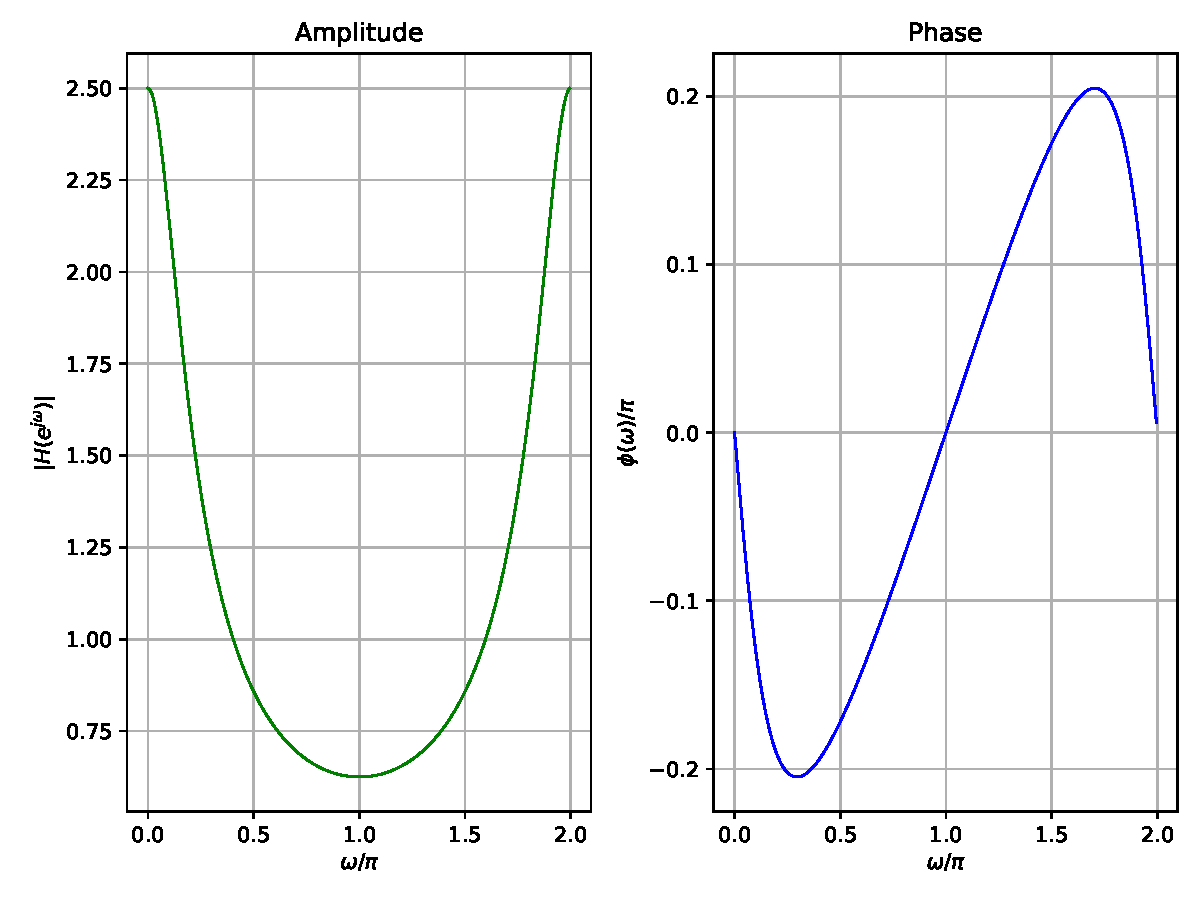
\includegraphics[width=16cm]{figure31.pdf}
	\caption{幅频特性和相频特性(Python)}\label{fig:figure31}
\end{figure}

\begin{figure}[htbp]
	\centering
	\begin{minipage}[t]{0.48\textwidth}
		\centering
		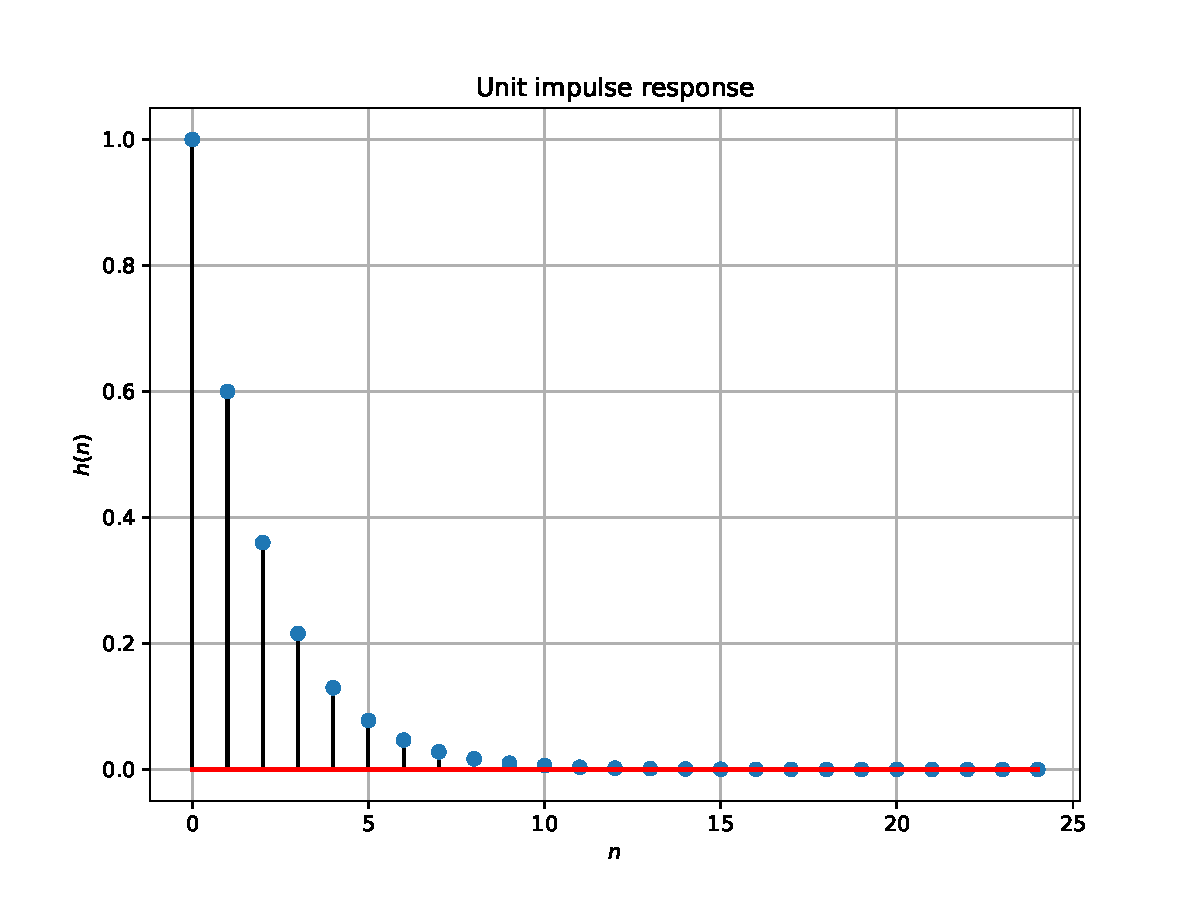
\includegraphics[width=6cm]{figure/impz11.pdf}
		\caption{单位脉冲响应(Python)}\label{fig:impz11}
	\end{minipage}
	\begin{minipage}[t]{0.48\textwidth}
		\centering
		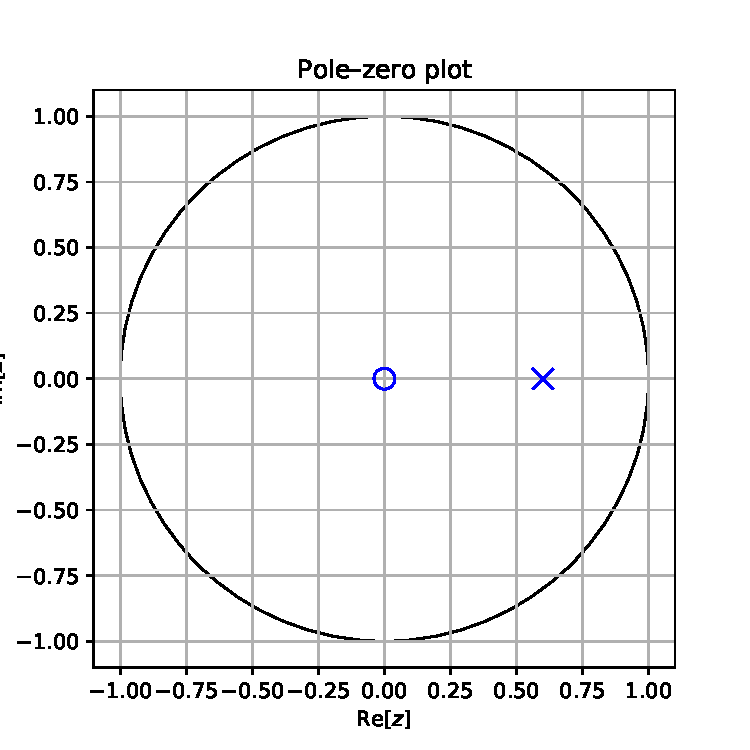
\includegraphics[width=6cm]{figure/zplane11.pdf}
		\caption{零极点分布图(Python)}\label{fig:zplane11}
	\end{minipage}
\end{figure}

\begin{lstlisting}[language=Python]
# 幅频特性和相频特性
a = np.array([1,-0.6])
b = np.array([1, 0])

omega, H = signal.freqz(b, a, whole=True)

plt.figure(figsize=(8, 6), dpi=80)

plt.subplot(121)
plt.plot(omega/np.pi, np.abs(H), 'g', linewidth=1.0)
plt.grid()
plt.xlabel('$\omega/\pi$')
plt.ylabel('$|H(e^{j\omega})|$')
plt.title('Amplitude')

plt.subplot(122)
plt.plot(omega/np.pi, np.angle(H)/np.pi, 'b', linewidth=1.0)
plt.grid()
plt.xlabel('$\omega/\pi$')
plt.ylabel('$\phi(\omega)/\pi$')
plt.title('Phase')

plt.tight_layout()
plt.show()
\end{lstlisting}

\begin{lstlisting}[language=Python]
# 单位脉冲响应
n, h = signal.dimpulse((b,a,1),n=25)
plt.figure(figsize=(8, 6), dpi=80)
plt.stem(n, np.squeeze(h), linefmt='black',  basefmt='r-', markerfmt="C0o")
plt.grid()
plt.xlabel('$n$')
plt.ylabel('$h(n)$')
plt.title('Unit impulse response')
plt.show()
\end{lstlisting}

\begin{lstlisting}[language=Python]
# 零极点分布图
from matplotlib.patches import Circle

z, p, k = signal.tf2zpk(b, a) # 求极点零点

fig, ax = plt.subplots(figsize=(5,5))
circle = Circle(xy=(0.0, 0.0), radius=1, fill=False, color='black')
ax.add_patch(circle)

plt.plot(p.real, p.imag, 'bx', markersize=10)
plt.plot(z.real, z.imag, 'o', markersize=10, color='none', markeredgecolor='b')
plt.grid()

r = 1.1 * np.amax(np.concatenate((abs(z), abs(p), [1]))) # z, p 模值和 1 的最大值乘以 1.1
plt.xlabel('$\mathrm{Re}[z]$')
plt.ylabel('$\mathrm{Im}[z]$')
plt.title('Pole–zero plot')
plt.axis([-r, r, -r, r])
plt.show()
\end{lstlisting}

\section{总结}

\subsection{杨文韬}

主要负责 \LaTeX 排版和所有代码的 Python 版本重写。

\begin{itemize}
\item 问题1:在 Python 中如何求 DTFT?

思路:一种方法是直接模拟,生成序列根据公式直接计算;另一种方法是其形式是有理多项式时可以通过库函数 \lstinline[language=Python]|scipy.signal.freqz| 求解。
\item 问题2:如何绘制零极点图?

思路:在 MATLAB 中可以通过 \lstinline[language=Matlab]|zplane()| 函数直接获得。在 Python 中可以通过库函数 \lstinline[language=Python]|scipy.signal.tf2zpk| 获得零点和极点,调用 \lstinline[language=Python]|matplotlib.patches| 库里的函数生成圆再绘制零极点。
\end{itemize}

\subsection{刘浩}

主要负责 \ref{sec:matlab1} 部分 MATLAB 代码编写。

\begin{itemize}
\item 问题1:matlab 如何将多个效果图放到一起显示?

解决方法:经查询资料后学会用 \lstinline[language=Matlab]|subplot| 函数确定图像放置位置
\item 问题2:如何使用 matlab 得到序列的幅频和相频特性?

解决方法:使用 \lstinline[language=Matlab]|abs| 函数获得幅度的绝对值,使用 \lstinline[language=Matlab]|angle| 函数获得序列的相位特性
\item 问题3:获得的图像显示不全怎么办?

解决方法:使用 \lstinline[language=Matlab]|axis| 函数调整横纵坐标轴可以获得更好的图像显示效果
\end{itemize}

\subsection{周泽熙}

主要负责 \ref{sec:matlab2} 部分 MATLAB 代码编写。

\begin{itemize}
\item 问题:如何通过差分方程求解频率响应?

在查阅相关库函数后,发现信号处理包中自带 \lstinline[language=Matlab]|freqz()| 函数可用于求解。在使用时仅需传入差分方程两侧系数,便能得到频率响应。再通过 \lstinline[language=Matlab]|abs()| 和 \lstinline[language=Matlab]|angle()| 求模和角度,便可得到幅频特性和相频特性。
\end{itemize}

% % 参考文献,此处以 MLA 引用格式为例

%\begin{thebibliography}{9}
%\end{thebibliography}

% % \includepdf[pages={1,2}]{Memo.pdf} 
% 可以直接导入pdf页面
%\newpage
%\begin{appendices}  % 附录环境
%\section{核心层}\label{subsec:B}
%\end{appendices}

\end{document}  % 结束